% -*- coding: UTF8 -*-
% firstDocument.tex
% tex的第一个文档
% XelaTex 命令编译

% ---引用包---

% 中文article包,使用UTF8编码
\documentclass[UTF8]{ctexart}
% 支持多种语言输入
% \usepackage[greek,english]{babel}
% 插图功能宏包
\usepackage{graphicx}
\usepackage{float}
\usepackage{amsmath}
% 设计页面尺寸的宏包
\usepackage{geometry}
% 改变图表标题格式的宏包
\usepackage[format=hang, font=small, textfont=it]{caption}
% 代码高亮
\usepackage{minted}


% ---导言区---
% \begin{document}前的部分为导言区(preamble),导言区通常用来对文档的性质做一些设置

% ------声明内容-------

% 定义a4纸,版心居中,长宽占页面的80%
\geometry{a4paper, centering, scale=0.8}

% \bibliographystyle声明参考文献格式
\bibliographystyle{plain}

% ------自定义内容-------

% \newtheorem定义新定理
\newtheorem{thm}{定理}

% \newcommand设置新命令
\newcommand\degree{^\circ}

% \newenvironment定义新环境
\newenvironment{myquote}
  {\begin{quote} \kaishu \zihao{-5}}
  {\end{quote}}

% ------预定义内容-------

% 以下内容并不会马上编译,而是在\maketitle处编译
\title{\heiti tex的教学文档}
\author{\kaishu 操杰朋}
\date{\today}


% ---正文部分---
\begin{document}

\maketitle

% \tableofcontents命令输出目录
\tableofcontents

\section{基础部分}

% 汉字后面的空格会被忽略,其它符号后面的空格则保留
left right 左 右\footnote{这是一个脚注}

% 使用空行分段,当个空行并不会使文字灵气一段,空白行则会另起一段
这是另起一行\emph{这里是强调}

% 行内公式(inline formula),正文公式(in-text formula)
$a + b \times 90^\circ + 90\degree$

% 列表公式(displayed formula)
\begin{equation}
  a(b + c) = ab + ac
\end{equation}

\begin{equation}\label{eq:gougu}
  AB^2 = BC^2 + AC^2
\end{equation}

文字文字
% 插入图片,第一个参数为图形宽度,第二个为图片地址(支持pdf,png,jpg,eps等)
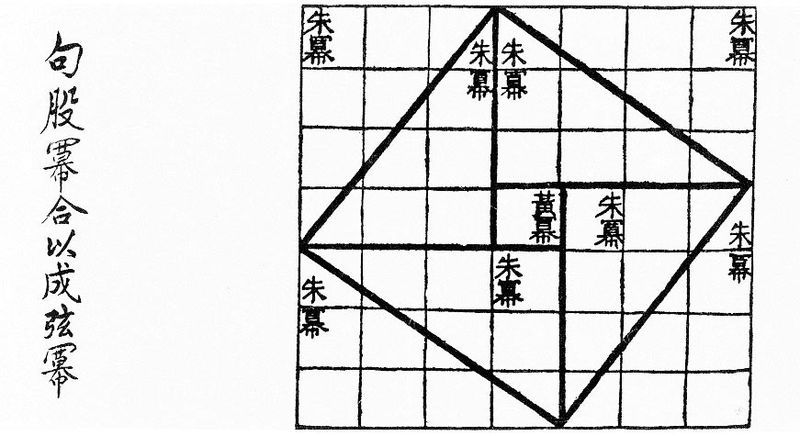
\includegraphics[width=3cm]{1.jpg}
文字文字

图\ref{flag:xiantu} 是一张图片引用

%figure即插图使用的浮动体环境[ht]表示here or top
\begin{figure}[ht]
  \centering
  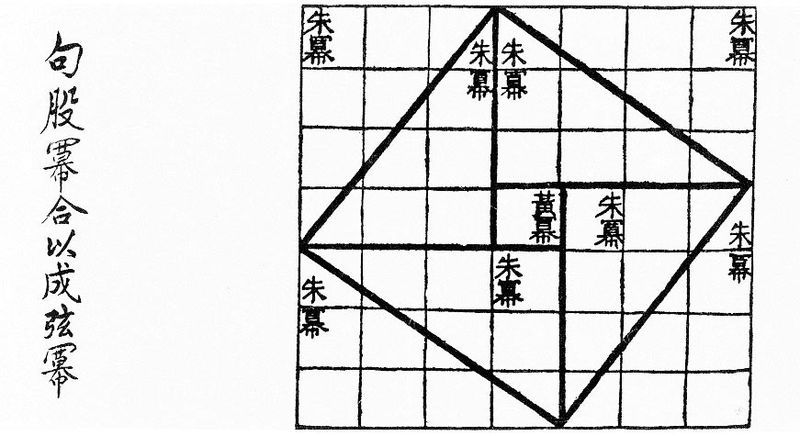
\includegraphics[scale=0.5]{1.jpg}
  \caption{一张图片}
  % 使用该标签可以在文章的其他地方引用\caption产生的编号
  \label{flag:xiantu}
\end{figure}

% \eqref 专门用于公式的引用,由package amsmath提供
满足式 \eqref{eq:gougu}的整数称为 \emph{勾股数}。

\begin{quote}
  % \zihao设置字号 \kaishu即楷书
  \zihao{-5} \kaishu 这里是引用
\end{quote}

\begin{myquote}
  这里是自定义引用
\end{myquote}

\begin{abstract}
  这里是摘要
\end{abstract}

\begin{thm}[测试定理]
  这里是自定义定理
  % --将输出"en dash",即与字母"n"相当的短线
    7--8
\end{thm}

% 表格|rrr|表示表格三列,都是右对齐
\begin{tabular}{|rrr|}
\hline
    直角边$a$ & 直角边$b$ & 斜边$c$ \\
\hline
    3 &  4 &  5 \\
    5 &  12 & 13 \\
\hline
\end{tabular}

% h表示不浮动[H],[H]是由package float提供
\begin{table}[H]
  \begin{tabular}{|rrr|}
    \hline
        直角边$a$ & 直角边$b$ & 斜边$c$ \\
    \hline
        3 &  4 &  5 \\
        5 &  12 & 13 \\
    \hline
  \end{tabular}
  % \qquad 表示 2em(em表示equal M)
  \qquad ($a^2 + b^2 = c^2$)
\end{table}

文献引用 \cite{Kline}

% \notice会在列表中显示并不直接引用的文献,一般写在\bibliography前
\nocite{Shiye}
\bibliography{math}

\section{文本部分}
% 重音命令
\begin{table}[H]
\begin{tabular}{cccc}
\hline
\`o & \'o & \^o & \"o \\
\~o & \=o & \.o & \u{o} \\
\v{o} & \H{o} & \t{oo} & \r{o} \\
\c{o} & \d{o} & \b{o} & \\
\hline
\end{tabular}
\end{table}

% 特殊字符
\begin{table}[H]
\begin{tabular}{cccc}
\hline
\AA & \aa & \AE & \ae \\
\OE & \oe & \SS & \ss \\
\IJ & \ij & \L & \l \\
\O & \o & \i & \j \\
\hline
\end{tabular}
\end{table}

% 输入希腊字母,由宏包babel提供
% \textgreek{abcde}

% 取消连字
shelfful shelf{}ful shelf\/ful

\begin{minted}{c}
int main()
{
  printf("hello world");
  return 0;
}
\end{minted}

\end{document} 